% Computer Architecture (4190.308) Fall 2016 
% Seoul National University CARES Lab
% Lab 4 documentation

% Lines that need modification : 24~27, 55~56 (location of files)

\documentclass{article}
\usepackage{graphicx, caption, subcaption, verbatim, moreverb, alltt, algorithm2e, kotex}
\usepackage[protrusion=true,expansion=true]{microtype}
\usepackage{fancyvrb}
\DeclareGraphicsExtensions{.pdf,.png,.jpg}
\let\verbatiminput=\verbatimtabinput

\setlength{\oddsidemargin}{0.25in}	% 1.25in left margin 
\setlength{\evensidemargin}{0.25in}	% 1.25in left margin (even pages)
\setlength{\topmargin}{0.0in}		% 1in top margin
\setlength{\textwidth}{6.0in}		% 6.0in text - 1.25in rt margin
\setlength{\textheight}{9in}		% Body ht for 1in margins
\addtolength{\topmargin}{-\headheight}	% No header, so compensate
\addtolength{\topmargin}{-\headsep}	% for header height and separation

\begin{document}

\title{Lab 4 : Four-stage Multicycle Processor Implementation}   % type title between braces
\author{CSE 4190.308 Computer Architecture \\ 2 Exercises (Total 70 Points) }         
\date{Received: April 23, 2016 \\Due: 11:00 a.m., April 30, 2016\\ \ \\ TA Office
Hours: 7:00 - 8:00 p.m., 4/28 4/29}    % type date between braces
\maketitle

\section{Introduction}

This lab examines processor implementation in Bluespec. You will begin with a two-stage Y86-64
processor. For this lab, the first part of the lab requires you to implement a list of missing instructions 
and run a series of tests to validate the design. The second part of the lab requires you to divide 
the two-cycle implementation into a multi-stage non-pipelined version.
This document describes the processor infrastructure, including how to build and run the processor 
to determine if it functions correctly and how well it performs, advice on how to debug the
processor, the initial processor design, and detailed steps you should take to successfully implement
the missing instructions.

\subsection{Lab Organization}
In the processor module used by your Lab 4 model, the file \texttt{Proc.bsv} describes the
processor architecture. Figure 1 shows a rough sketch of the microarchitecture. 
There is a buffer register between the instruction fetch
stage and Decode-Execute-Writeback stage. For this lab, all your code changes will be limited to two
files: \texttt{Decode.bsv}, which implements the decode method used by the processor
core, and \texttt{Proc.bsv}, two-stage multicycle processor.

\begin{figure}[htbp]
	\begin{center}
		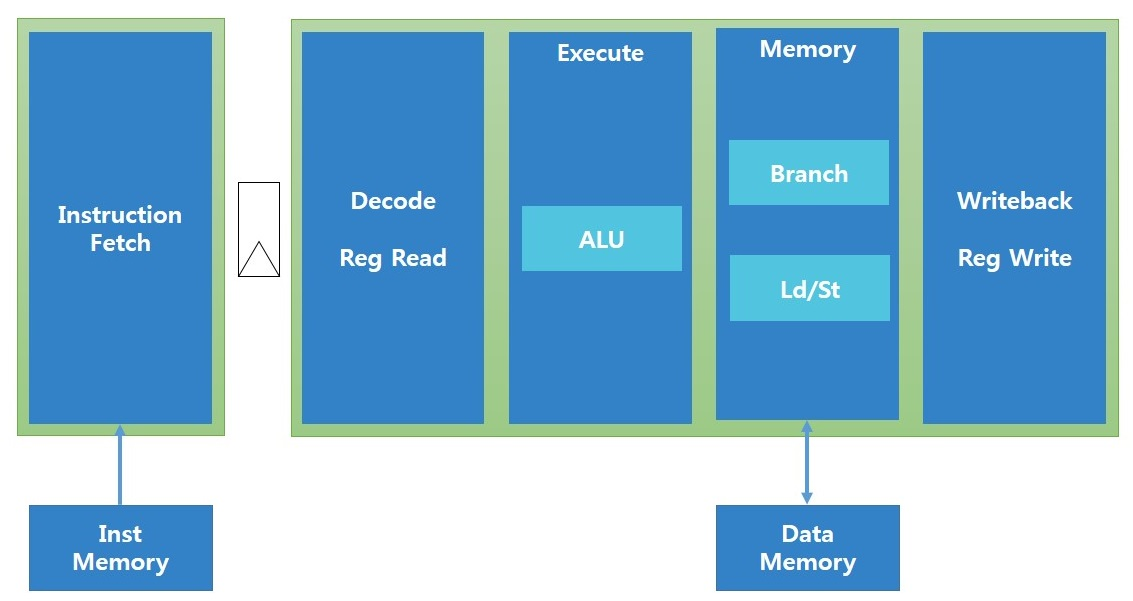
\includegraphics[scale=0.4]{figure1.jpg}
		\caption{Two-stage Architecture Y86-64 Processor} \label{fig:lable}
	\end{center}
\end{figure}
The Y86-64 Instruction Set Specification can be found in the PDF file, \texttt{Chapter 5} available
from the ‘LECTURE NOTE’ menu of the course webpage. 

\section{Getting Started}
(If you need a language assistance, please see our English-speaking TAs.)
\subsection{How to Download the Source Code}
컴퓨터 구조 과목에서 사용하게 될 모든 실습은 이전에도 언급되었듯이 svn 서버를 통해 관리됩니다.
Lab 4의 실습 코드를 받는 방법은 기존 Lab들과 동일합니다.
수업 홈페이지에 올라와 있는 \texttt{add-lab4.sh} 스크립트를 다운받고,
이전 Lab을 수행했던 실습 디렉터리의 상위에 위치시킵니다.

\begin{Verbatim}[frame=single]
   $ ls
   add-lab4.sh YOUR_ID/
   $ ls YOUR_ID/
   lab0/ lab1/ lab2/ lab3/
\end{Verbatim}

그 후 아래 예제와 같이 본인의 ID를 인자로 스크립트를 실행하셔야 합니다.
이 아이디는 첫 실습 과제에 앞서 \texttt{student-create.sh} 스크립트로 생성했던 아이디입니다.
코드를 다운 받는 과정에서 archi16의 password를 요구할 경우 강의 홈페이지와 동일한 비밀번호를 입력하시면 됩니다.
\\\\
\indent다음으로, svn 계정의 비밀번호를 입력해야 이 과정을 무사히 마칠 수 있습니다.
svn 계정의 아이디는 \texttt{student-create.sh} 스크립트로 생성했던 아이디이며, 
비밀번호는 공지한 바와 같이 조교에게 이메일로 보내주신 희망 비밀번호로 설정되어 있습니다.

\begin{Verbatim}[frame=single]
   $ ./add-lab4.sh YOUR_ID
   Getting source codes for YOUR_ID
   archi16@hyewon.snu.ac.kr's password: 
   ...
   Checking in initial repository
   Authentication realm: <svn://hyewon.snu.ac.kr:3690> 2016 Computer Architecture
   Password for 'YOUR_ID': 
   ...
   Transmitting file data .....
   Committed revision 14.
\end{Verbatim}

위와 같이 새로운 revision 번호를 알려주는 메세지가 보이면 실습 코드 다운이 완료된 것입니다. 
실습 디렉터리 아래에 \texttt{lab4} 디렉터리가 새롭게 생성되었을 것입니다.

\begin{Verbatim}[frame=single]
   $ ls YOUR_ID/
   lab0/ lab1/ lab2/ lab3/ lab4/
\end{Verbatim}

\subsection{Directory Structure of Lab 4}
Lab 4 실습의 디렉터리 구조는 다음과 같습니다.

\begin{Verbatim}[frame=single]
lab4/	
    build/
    lib/
       common-lib/
                  ProcTypes.bsv
    src/
       Decode.bsv
       Proc.bsv 
       decode_result.orig
       y86
\end{Verbatim}

\begin{description}
\item [\texttt{build/}]\hfill \ \\
	%
	컴파일 시 생성되는 파일들이 위치하는 폴더입니다.

\item [\texttt{lib/}]\hfill \ \\
	% 
	실습에 사용되는 library 파일들이 위치하는 폴더입니다.
	실습을 하면서 수정할 필요 없는 Bluespec 소스 파일들을 포함하고 있습니다.

\item [\texttt{lib/common-lib/ProcTypes.bsv}]\hfill \ \\
	% 
	Y86-64 프로세서의 타입을 지정해둔 파일입니다. 이 파일을 참조하여 앞으로 프로세서 관련
	Lab에서 쓰일 Type들의 정의를 볼 수 있습니다. 

\item [\texttt{src/Decode.bsv}]\hfill \ \\ 
	%
	Y86-64 프로세서에서 80bit 명령어를 Decoding하는 것에 대한 모듈입니다. Exercise 1에서 
	고치게 될 파일입니다. 

\item [\texttt{src/Proc.bsv}]\hfill \ \\
	%
	위에서 구현한 두 모듈을 import하여 프로세서를 구현하는 파일입니다. Exercise 2에서 
	고치게 될 파일입니다. 

\item [\texttt{src/decode\_result.orig}]\hfill \ \\
	%
	디코딩 결과의 모범답안 입니다. 구현한 디코딩 로직의 검증 결과로 생성되는
	\texttt{decode\_result}와 diff명령을 통하여 비교를 하면 로직을 정상적으로 구현하였는지
	확인할 수 있습니다. 

\item [\texttt{src/y86}]\hfill \ \\
	Exercise 1, 2에서 구현할 프로세서에 대해 컴파일 및 검증을 할 수 있도록하는 스크립트 파일입니다.

\end{description}

\subsection{How to Simulate the Design}
Lab 4는 크게 디코딩 로직의 구현과 two-stage multi-cycle 프로세서를 four-stage multi-cycle 프로세서로
 변환하는 과제로 나눠집니다.
 
 \subsubsection{Compiling and Simultation in Exercise}
 구현할 디코딩 로직과 four-stage multi-cycle 검증은 아래와 같이 \texttt{y86}
 스크립트를 실행하여 이뤄집니다. 
\begin{Verbatim}[frame=single]
    $ ./y86 -c [-d]
    $ ./y86 -r [-d]
\end{Verbatim}
\noindent먼저, -c 플래그로 구현한 Y86-64프로세서를 컴파일을 할 수 있습니다.
다음, -r 플래그로 모든 명령어 수행을 테스트하거나, \texttt{-o} 플래그를 통해 특정 명령어를
테스트할 수 있습니다. 각 명령어 테스트가 끝나면, PASS 여부 및 수행한 사이클과 명령어 수가 출력됩니다.\\
\noindent-d 플래그를 추가로 주면 디코드 테스트를 위한 컴파일과 명령어 수행을 할 수 있습니다.
\noindent테스트 디코딩 수행 결과는 \texttt{src}폴더내에
\texttt{decode\_result}라는 텍스트 파일이 저장되고, 이 파일을 제공되는 올바른
결과인 \texttt{decode\_result.orig} 
파일과 비교하여 디코딩 로직이 제대로 구현됐는지 확인 할 수 있습니다. 참고로, Linux에서 아래와 같은
명령어를 이용하면, 생성되는 \texttt{comp}파일에서 두 파일의 다른 점을 비교할 수 있습니다.
\begin{Verbatim}[frame=single]
    $ diff decode_result decode_result.orig > comp 
\end{Verbatim}

\section{Implementing Decoding Module}

\texttt{lab4/src/Decode.bsv} 의 decode 함수는 80bit의 명령어를 정해진 형식에 따라 디코딩하는 함수입
니다. 디코딩 결과는 \texttt{ProcType.bsv}에 정의돼있는 \texttt{DecodedInst}와 같습니다.
valA, valB, copVal 필드는 디코딩 이후 사용되는 필드로 Decode에서 설정하지 않습니다.

\begin{Verbatim}[frame=single]
	typedef struct{
		IType   iType;
		OpqFunc opqFunc;
		CondUsed  condUsed;
		Addr valP;
		Maybe#(FullIndx) dstE;
		Maybe#(FullIndx) dstM;
		Maybe#(FullIndx) regA;
		Maybe#(FullIndx) regB;
		Maybe#(Data) valA;
		Maybe#(Data) valB;
		Maybe#(Data) valC;
		Maybe#(Data) copVal;
	} DecodedInst deriving(Bits,Eq);
\end{Verbatim}

\noindent{\bf IType iType}\\
명령어의 타입을 나타냅니다. 마찬가지로 \texttt{ProcType.bsv}에 정의 되어 있습니다. \texttt{Mfc0, Mtc0}에
대해서는 이미 구현이 되어있으므로 이 과제에서는 무시해도 무방합니다.

\begin{Verbatim}[frame=single]
	typedef enum{
		Unsupported,
		Rmov,
		Opq,
		RMmov,
		MRmov,
		Cmov,
		Jmp,
		Push,
		Pop,
		Call,
		Ret,
		Hlt,
		Nop,
		Mtc0,
		Mfc0 
	}IType deriving(Bits, Eq);
\end{Verbatim}

\noindent{\bf OplFunc oplFunc}\\
디코딩 되는 명령어가 어떤 종류의 Opq 연산을 사용하는지를 나타냅니다. 마찬가지로 \texttt{ProcType.bsv}
에 정의 되어 있습니다.

\begin{Verbatim}[frame=single]
	typedef enum{
		FNop,
		FAdd,
		FSub,
		FAnd,
		FXor
	} OplFunc deriving(Bits, Eq);
\end{Verbatim}

\noindent{\bf CondUsed condUsed}\\
디코딩 되는 명령어가 어떤 종류의 Cond 연산을 사용하는지를 나타냅니다. 마찬가지로 \texttt{ProcType.bsv}에 정의 되어 있습
니다.

\begin{Verbatim}[frame=single]
	typedef enum{
		Al,   // Unconditional
		Eq,   // Equal
		Neq,  // Not Equal
		Lt,   // Less than
		Le,   // Less than or Equal
		Gt,   // Greater than
		Ge    // Greater than or Equal
	} CondUsed deriving(Bits, Eq);
\end{Verbatim}

\noindent{\bf Addr valP}
\\다음 실행할 명령어 주소를 나타냅니다.
\\\\\noindent{\bf Maybe\#(Fullindx) dstE}
\\Destination 레지스터의 번호를 나타냅니다.
\\\\\noindent{\bf Maybe\#(Fullindx) dstM}
\\메모리에서 값이 로드될 Destination 레지스터 번호를 나타냅니다.
\\\\\noindent{\bf Maybe\#(Fullindx) regA}
\\첫 번째 Source 레지스터의 번호를 나타냅니다.
\\\\\noindent{\bf Maybe\#(Fullindx) regB}
\\두 번째 Source 레지스터의 번호를 나타냅니다.
\\\\\noindent{\bf Maybe\#(Data) valC}
\\명령이 immediate 값을 사용할 경우, 사용할 immediate 값을 나타냅니다.
\\\\
디코딩을 올바르게 수행하기 위하여, \texttt{decode}함수 안의 \texttt{case} 문에 있는 경우마다 정확한 값을
위에 설명한 필드마다 채워 넣어야 합니다. 경우마다 디코딩된 명령이 참고할 필드만 신경써서 채우면 되고, 꼭 모든 필드 마다 새로운 값을 넣을 필요는 없습니다.
\\예를 들어 \texttt{mrmovq}와 같은 명령어
는 \texttt{valC} 값을 사용하지만, \texttt{cmov}와 같은 명령어는 \texttt{valC} 값을 사용하지 않습니다. 따라서
\texttt{cmov}와 같은 경우, \texttt{valC}는 \texttt{Invalid}로 설정하지만, \texttt{mrmovq}의 경우에는 
\texttt{valC}의 필드에 정확한 값을 설정해주어야 합니다. 이와 같이 각 명령 마다 \texttt{DecodedInst}의 필드가 어떻게 사용되는지를 확실하게 숙지하고, 필요한 필드를 새로 설정하여야 합니다.
\\\\
\noindent수정해야할 \texttt{decode} 함수의 구조는 아래와 같습니다.

\begin{Verbatim}[frame=single]
function DecodedInst decode(Inst inst, Addr pc);
	DecodedInst dInst = ?;
	let iCode = inst[79:76]; 
	let ifun  = inst[75:72];
	let rA    = inst[71:68];
	let rB    = inst[67:64];
	let imm   = little2BigEndian(inst[63:0]);
	let dest  = little2BigEndian(inst[71:8]);

	case (iCode)
	halt, nop :
	begin
		...
	end
	irmovq :
	begin
		...
	end
	...
	endcase
	return dInst;
endfunction
\end{Verbatim}

  리턴 값인 \texttt{dInst}의 초기화 이후에, \texttt{inst} 인자를 \texttt{bit concatenate}
함수를 이용하여 필요한 값들을 설정해놓았습니다. 따라서 나머지 디코딩 모듈 구현을 위해서는
\texttt{inst}는 다시 참조할 필요가 없고, 새로 설정된 값들이 의미하는 바가 무엇인지를 이해하고 새로운
리턴 값을 만드는데 사용하면 됩니다.
\\\\
  \indent\texttt{case} 문은 \texttt{iCode} 에 따라 \texttt{dInst}의 필드를 재설정해주는 방식으로 되어있습니다.
올바른 디코딩 모듈의 구현을 위해, 명령어에 따라 설정해야할 필드가 무엇인지를 이해하여 모든 명령어에 대해 빠짐없이 정확한 필드값을 설정해야 합니다.

\noindent \paragraph{\bf Exercise [1] (30 points):} \texttt{Decode.bsv} 파일 안의 decode함수를 완성하시오. 다음 Exercise로
넘어가기 전에 반드시 \texttt{y86} 스크립트를 통해 결과를 확인할 것.

\section{Multi-cycle Y86-64 implementation}

The provided code implementes a two-cycle non-pipelined Y86-64
implementation. Your goal for this lab is to split one of the stages
into three stages, making the processor a four-cycle non-pipelined
implementation.

Inside the provided \texttt{Proc.bsv} file, you can find the module
\texttt{mkProc}, which implements two rules \texttt{doFetch} and
\texttt{doExecute}. These rules are scheduled one after another by
setting the register \texttt{stage} of type \texttt{Stage}. Your job
is to split the \texttt{doExecute} rule into three rules:
\texttt{doExecute}, \texttt{doMemory} and \texttt{doWriteBack}. You
can add these stages into the \texttt{Stage} type by adding them to
the \texttt{typedef enum} statement.

The \texttt{doExecute} stage should take care of \texttt{decode} and
\texttt{execute}. The \texttt{doMemory} stage should take care of the
\texttt{dMem} requests, and \texttt{doWriteBack} stage should take
care of the writeback to \texttt{rf}.

In order to reduce the cycle count, another requirement is to skip the
\texttt{doMemory} stage whenever it is not needed. So when there is no
memory access instructions, the processor should behave as a
three-stage non-pipelined processor.

\noindent \paragraph{\bf Exercise [2] (40 points):} Divide the \texttt{doExecute}
rule into \texttt{doExecute}, \texttt{doMemory} and
\texttt{doWriteBack}, to make the processor a four-cycle non-pipelined
implementation. The \texttt{doMemory} rule should be skipped
whenever it is not required. You can check the impact of your
modifications through the script output.

\end{document}
